\scanpage{77}
\mspage{6}
or tout chemin effectif $x\longrightarrow y$ (donné par une appl continue $[0,1]\longrightarrow X$) se décompose en \inserted{composé de} chemins \inserted{``directs''}
\diagram{\begin{tikzcd}[ampersand replacement=\&,column sep=small]
x_0=x \arrow[r,no head] \& x_1 \arrow[r] \& x_2 \cdots \arrow[r,no head] \& x_n=y
\end{tikzcd}}
entre \deleted{\unsure{chemins|chemin}} \inserted{points} ``proches''. Dans le cas \deleted{général}, \inserted{où les $X_\alpha$ sont fermés} un argument de descente (comme déjà signalé dans la première hypothèse) donne le résultat énoncé.

Cette deuxième démonstration a l'avantage de marcher également pour \inserted{montrer} le résultat un peu plus général, et peut-être plus intéressant du point de vue pratique, où pour $\unsure{\forall|\text{tt}}\alpha$ on a $I_\alpha\subset T_\alpha$ partie \inserted{non vide} de $T_\alpha$ (normalement, partie finie) de telle façon que pour $T_\alpha\subset T_\beta$ on ait $I_\alpha\subset I_\beta$ (normalement, on prend d'abord $I\subset X_K$ convenable et on prend $I_\alpha=I\cap T_\alpha$, donc $I=\bigcup I_\alpha$), et on se borne aux $g^\alpha_{y,x}$ pour $x,y\in I_\alpha$: leur connaissance permet de retrouver \uline{tous} \inserted{$f_l(u)$,} $g_{\deleted{\unsure{yx}}l}(u)$, $l$ un chemin quelconque dans

\margin{On a deux façons de ``récupérer'' l'opération de $\Gamma$ sur le groupoïde $\widehat{\Pi}_1(X,I)$ (où $I\subset X_K$) en quelque sorte duales l'une de l'autre: soit on prend \unsure{un syst.} de $l_j:x_j\mathbin{-}y_j$ $(x_j,y_j\in I)$ générateurs pour $\Pi_1(X,I)$, et regarde les $f_{l_j}(u)$ ou $g_{l_j}(u)$, soit on fixe des $T_\alpha$ comme dessus, et on regarde les $g^\alpha_{x,y}$ $(\alpha\in A,x,y\in T_\alpha\cap I)$. En fait on voit que \unsure{très|trop} \unsure{bientôt} qu'il est \deleted{\unsure{ff}} inutile de supposer que les $T_\alpha$ \unsure{recouvrent|recouvrir} $X$ (p.ex. si les $T_\alpha$ sont les supports des chemins \unsure{$l_j$}).}

\figure{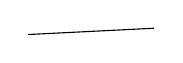
\begin{tikzpicture}\draw (0,0)--(1.6,.08);\end{tikzpicture}}
Jusqu'à présent, on a maintenu $u$ fixe, on a fait varier $l$, resp. $(T/X,x,y)$. Si on regarde ce qui se passe pour $u\in\Gamma$ variable, les formules
\margin{76}
